% This file was created with tikzplotlib v0.10.1.
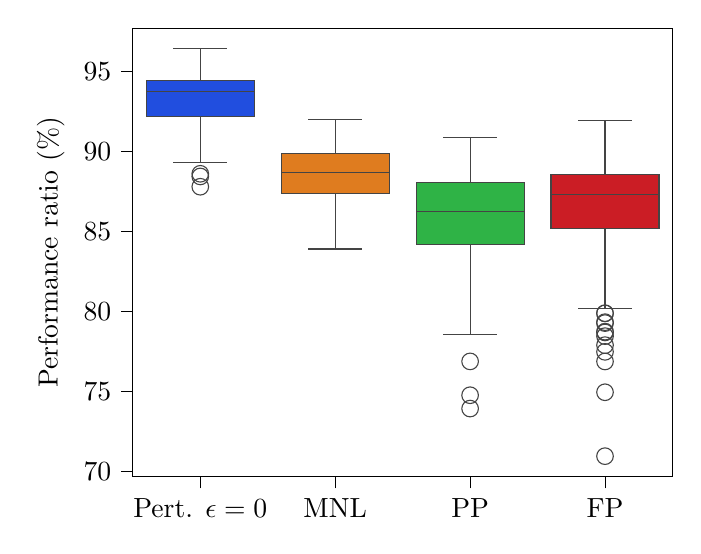
\begin{tikzpicture}

\definecolor{chocolate22312431}{RGB}{223,124,31}
\definecolor{darkgray176}{RGB}{176,176,176}
\definecolor{darkslategray68}{RGB}{68,68,68}
\definecolor{firebrick2032937}{RGB}{203,29,37}
\definecolor{limegreen4717970}{RGB}{47,179,70}
\definecolor{royalblue3378223}{RGB}{33,78,223}

\begin{axis}[
tick align=outside,
tick pos=left,
x grid style={darkgray176},
xmin=-0.5, xmax=3.5,
xtick style={color=black},
xtick={0,1,2,3},
xticklabels={Pert. \(\displaystyle \epsilon=0\),MNL,PP,FP},
y grid style={darkgray176},
ylabel={Performance ratio (\%)},
ymin=69.680673639012, ymax=97.6849116827857,
ytick style={color=black},
ytick={65,70,75,80,85,90,95,100},
yticklabels={
  \(\displaystyle {65}\),
  \(\displaystyle {70}\),
  \(\displaystyle {75}\),
  \(\displaystyle {80}\),
  \(\displaystyle {85}\),
  \(\displaystyle {90}\),
  \(\displaystyle {95}\),
  \(\displaystyle {100}\)
}
]
\path [draw=darkslategray68, fill=royalblue3378223]
(axis cs:-0.4,92.1550598873663)
--(axis cs:0.4,92.1550598873663)
--(axis cs:0.4,94.4320875086815)
--(axis cs:-0.4,94.4320875086815)
--(axis cs:-0.4,92.1550598873663)
--cycle;
\addplot [darkslategray68]
table {%
0 92.1550598873663
0 89.3141091510825
};
\addplot [darkslategray68]
table {%
0 94.4320875086815
0 96.411991771705
};
\addplot [darkslategray68]
table {%
-0.2 89.3141091510825
0.2 89.3141091510825
};
\addplot [darkslategray68]
table {%
-0.2 96.411991771705
0.2 96.411991771705
};
\addplot [black, mark=o, mark size=3, mark options={solid,fill opacity=0,draw=darkslategray68}, only marks]
table {%
0 88.4261860970828
0 88.5921491576229
0 87.7830848219175
};
\path [draw=darkslategray68, fill=chocolate22312431]
(axis cs:0.6,87.3560116562822)
--(axis cs:1.4,87.3560116562822)
--(axis cs:1.4,89.860462167285)
--(axis cs:0.6,89.860462167285)
--(axis cs:0.6,87.3560116562822)
--cycle;
\addplot [darkslategray68]
table {%
1 87.3560116562822
1 83.8944048329985
};
\addplot [darkslategray68]
table {%
1 89.860462167285
1 92.0054887151522
};
\addplot [darkslategray68]
table {%
0.8 83.8944048329985
1.2 83.8944048329985
};
\addplot [darkslategray68]
table {%
0.8 92.0054887151522
1.2 92.0054887151522
};
\path [draw=darkslategray68, fill=limegreen4717970]
(axis cs:1.6,84.1874064264844)
--(axis cs:2.4,84.1874064264844)
--(axis cs:2.4,88.0602755325824)
--(axis cs:1.6,88.0602755325824)
--(axis cs:1.6,84.1874064264844)
--cycle;
\addplot [darkslategray68]
table {%
2 84.1874064264844
2 78.5603102520858
};
\addplot [darkslategray68]
table {%
2 88.0602755325824
2 90.8559884182014
};
\addplot [darkslategray68]
table {%
1.8 78.5603102520858
2.2 78.5603102520858
};
\addplot [darkslategray68]
table {%
1.8 90.8559884182014
2.2 90.8559884182014
};
\addplot [black, mark=o, mark size=3, mark options={solid,fill opacity=0,draw=darkslategray68}, only marks]
table {%
2 74.7604296747939
2 76.8727589975359
2 73.9267979744025
};
\path [draw=darkslategray68, fill=firebrick2032937]
(axis cs:2.6,85.1576943161778)
--(axis cs:3.4,85.1576943161778)
--(axis cs:3.4,88.5320969158398)
--(axis cs:2.6,88.5320969158398)
--(axis cs:2.6,85.1576943161778)
--cycle;
\addplot [darkslategray68]
table {%
3 85.1576943161778
3 80.1794945097269
};
\addplot [darkslategray68]
table {%
3 88.5320969158398
3 91.9023604993431
};
\addplot [darkslategray68]
table {%
2.8 80.1794945097269
3.2 80.1794945097269
};
\addplot [darkslategray68]
table {%
2.8 91.9023604993431
3.2 91.9023604993431
};
\addplot [black, mark=o, mark size=3, mark options={solid,fill opacity=0,draw=darkslategray68}, only marks]
table {%
3 77.4704878638738
3 78.6815953415637
3 79.8698078235877
3 77.889348193281
3 79.3237171490251
3 79.8853904517332
3 78.7327256715275
3 79.2652786401799
3 70.9535935500926
3 76.8683844974797
3 78.4509166524302
3 74.9461209549858
};
\addplot [darkslategray68]
table {%
-0.4 93.7052431465881
0.4 93.7052431465881
};
\addplot [darkslategray68]
table {%
0.6 88.678655660778
1.4 88.678655660778
};
\addplot [darkslategray68]
table {%
1.6 86.2381039465492
2.4 86.2381039465492
};
\addplot [darkslategray68]
table {%
2.6 87.2927229959253
3.4 87.2927229959253
};
\draw (axis cs:0,62.6796141280686) node[
  scale=0.75,
  anchor=base,
  text=black,
  rotate=0.0
]{\bfseries 93.25};
\draw (axis cs:1,62.6796141280686) node[
  scale=0.75,
  anchor=base,
  text=black,
  rotate=0.0
]{\bfseries 88.51};
\draw (axis cs:2,62.6796141280686) node[
  scale=0.75,
  anchor=base,
  text=black,
  rotate=0.0
]{\bfseries 85.78};
\draw (axis cs:3,62.6796141280686) node[
  scale=0.75,
  anchor=base,
  text=black,
  rotate=0.0
]{\bfseries 86.18};
\draw (axis cs:-1,62.9596565085063) node[
  scale=0.75,
  text=black,
  rotate=0.0
]{\bfseries \textbf{Average:}};
\end{axis}

\end{tikzpicture}
